\chapter{Architectural Design}
\label{cha:arch}

\section{Overview}
\label{sec:overview}
This section aims at giving an overview of the architectural components of the application, starting with a high-level approach towards a more detailed and deeper level of the technologies. We will discuss how and why we have chosen the technologies that will be used in the development of the clients and what kind of back-end solution.
\newline Travlendar+ relies on \textit{Amazon Web Services} (AWS), a collection of cloud computing services handled by Amazon.com which offers, among other things, servers, storage and database. It hosts our application and lays the foundation for the client-server communication. Besides benefiting of high reliability and scalability, AWS's resources enable us to have a degree of flexibility that cannot be achieved through hosting with normal services and implementation of our own Web API in the traditional way.
Accessing the AWS services is really feasible thanks to the AWS SDK's available that helps to take out of coding the complexity of accessing them providing wrapped APIs in every major technology that could be used to implement the clients.
Furthermore, the mobile client-side will be implemented with Xamarin.Forms, a cross-platform UI toolkit abstraction that allows us to develop a great multi-platform solution (iOS and Android) in C\# with an excellent code-sharing approach.
The web application will be based on Angular.js and HTML5.
Angular.js is one of the most popular JavaScript frameworks for web applications, it allows to have a rapid development and its maintained by Google Engineers meaning that you will find reliable support if needed. It perfectly integrates with HTML5 and its fully compatibly with the MVVM design approach. Further details are provided in the following sections.

\section{Component view}
\label{sec:comp_view}

From a high-level point of view, the following components of the system can be identified:
\begin{description}
	\item[Client:] Implementation of the application that makes requests to the server and will be provided with a response. In Travlendar+ the clients will be the mobile application and the web application, that interacts with the server through REST APIs.
	\item[Web Server:] Software running on a server able to communicate with web application clients using the HTTP(S) protocol, known also as back-end.
	
	\item[Application Server:] This layer makes the workflow and the business logic for the client applications work. It will be implemented with AWS technologies interacting with a different component for each type of client.
	\item[Web Browser:] Application for retrieving and presenting web pages and applications.
	\item[Database:] This layer handles retrieval and storage of data. It will be queried by the application server. This layer must guarantee ACID properties.
\end{description}

We list also the following components which may not strictly belong to the component view but play a key role in our design approach:
\begin{description}
	\item[AWS:] Cloud services that offer computing power, database storage, content delivery and other scalable functionalities.
	\item [AWS Cognito:] AWS component and client library that enables cross-device syncing of application-related user data.
	\item[Xamarin:] Framework that delivers native Android, iOS and Windows applications using a shared C\# codebase and same APIs.
\end{description}

These high-level components are laid down as follows.

\subsection*{Server-side application}
Since relying on AWS services, one of the main core service used is \textit{Amazon Cognito Sync}, a service which allows us to sync the user's data across multiple clients and platforms.
The login is managed by \textit{Amazon Cognito Identity} service and supports either the social platforms authentications (Facebook and Google) or the traditional email registration flow. This can be achieved by associating an identity with a dataset containing key-values pairs having a maximum size of 1 MB. Due to AWS limitations, each identity can be associated with maximum 20 datasets.
Amazon Cognito Sync functions by creating a local cache for the identity data. An interaction between the application and this local cache occurs when reading or writing the keys. 
This allows Travlendar+ to synchronize all the changes made on a device immediately to other devices.
Not only the user preferences are going to be stored but user events and means of transports too, this could be enhanced in future to other services using Amazon Cognito towards an AWS DynamoDB or and AWS Lambda if we would like to transfer some computational power towards the backend side. What's more, Amazon Cognito offers a scalable and modular way to react upon peaks in demands and traffic.

\begin{figure}
	\centering
	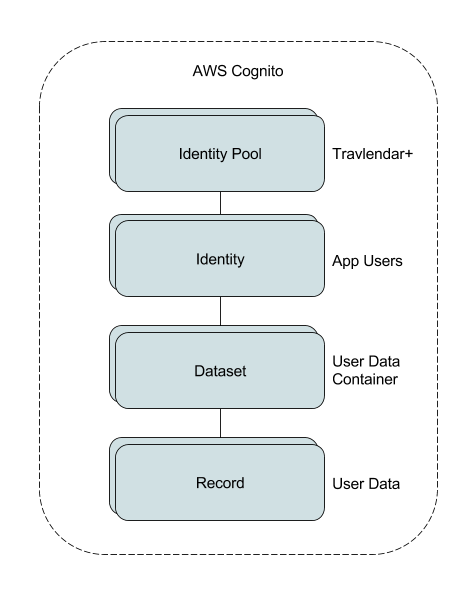
\includegraphics[width=6in]{./diagrams/CognitoDiagram.png}
	\caption{Structure of the Amazon Cognito Sync service.}
	\label{fig:seqCognito}
\end{figure}

\subsection*{Web Server}
The \textbf{mobile application} will interface with the application server through the wrapped RESTful APIs while the \textbf{web application} will run on a web server based on an Amazon Elastic Cloud Computing instance.
Amazon Cognito Sync will play a key role providing a real-time synchronization of the user data and event across the clients.
It provides a service of identity management within an identity pool, giving secure access to AWS services from all the platforms and synchronizing user's data. 
The data is persistent to the local storage first, making it available regardless the connectivity.

The web application will have a server to filter the request from the clients. 
It's based mainly on Amazon Web Application Firewall (AWS WAF).
AWS WAF will help to lower the load on the infrastructure (Layer 3 and Layer 4) from DDoS attack or other techniques and giving control over which traffic to allow or block. 
Includes full-featured API that can be used to create and/or deploy web security rules.
The runtime environment will be operating on Node.js that simplifies the development of the web application thanks to a rich and various JS modules. 
Besides that, we will use nginx on our Amazon EC2 instances to proxy the network traffic to the running Node.js instances.
It supports sophisticated Layer 7 load balancing as well as reverse proxy capabilities allowing a multiple web server infrastructure making the application more reliable.

\subsection*{Mobile client application}
Travlendar+ mobile application is thought to be implemented with Xamarin technologies. In addition to being an extremely powerful set of frameworks, it allows us to have a multi-platform presence and speed a little bit up the development phase while maintaining a high degree of modularity.
As a result, since these technologies make use of C\#, .NET SDKs is used. Particularly, Xamarin.Forms framework is used, which is, as said above, a cross-platform UI toolkit that allows us to create a native interface. While it is widely used and gained considerable fame since the very first release, Xamarin.Forms is still quite a new technology so whenever we need to build particular details whose APIs that abstract the platform may not exist, we plan to bind the native Android and iOS components by ourselves. So, we can choose to use the main control groups to create the User Interface, which are Pages, Layouts, Views and Cells that are mapped and rendered to the native equivalent and, indeed, Xamarin.iOS and Xamarin.Android are taken into account when customizing a platform-specific UI component. Xamarin.Forms applications are drawn up in the same way as any other cross-platform application. There are two viable approaches, the most common is with Portable Class Libraries (PCL) while the other is via Shared Projects.
Our choice is more directed towards the PCL that may result in a DLL usable on the specific platforms for which we provide support. Figure \ref{fig:pcld} shows the architecture of a cross-platform application using a PCL to share code. This approach has a number of advantages like a centralized code base consumed by the platform projects, refactoring operation affects all the code within the solution and the relief of referencing itself against the platform projects. 
The drawback may concern platform specific libraries, which cannot be referenced inside the PCL, but this can be avoided with the Dependency Injection pattern, using an interface in the Portable Class passing platform-specific features.

\begin{figure}
	\centering
	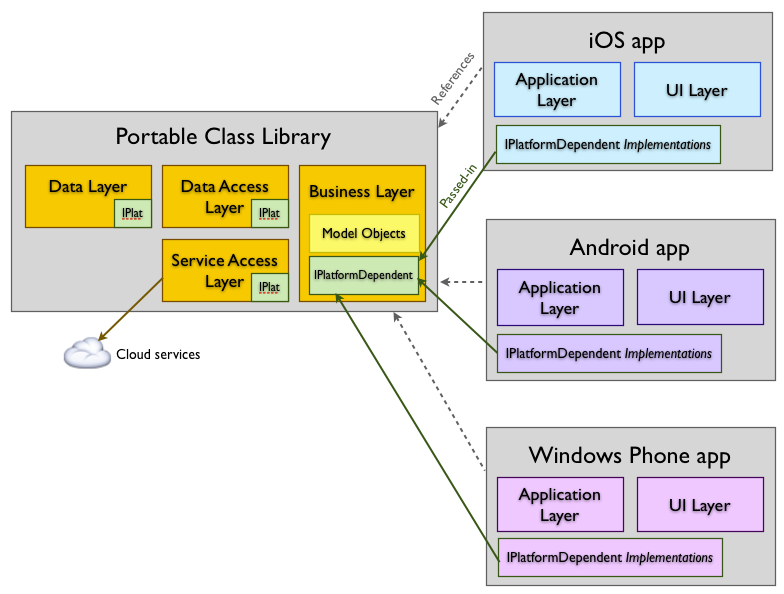
\includegraphics[width=6in]{diagrams/PCLDiagram.png} 
	\caption{PCL Diagram\cite{pcl}.}
	\label{fig:pcld}
\end{figure}

\subsection*{Web application}
As regards the web application, in order for it to be dynamic and highly responsive, the implementation consists of using the fifth standard of HTML enhanced by a structural framework, AngularJS, which indeed lets us compose HTML templates. The functionalities of the web application are almost the same of the mobile one, thus allowing real-time synchronization among the devices. The application is meant to be composed of component classes that manage the HTML templates and the business logic is implemented in services, boxing them in modules. We continue relying on the AWS SDK as for the mobile client application to implement the synchronization of the user data within the web one. 
AWS Cognito still plays a major role. This introduces an extra layer of abstraction from the back-end service, keeping the more sensitive pieces out of the exposed JavaScript.
The web application is hosted on the AWS infrastructure having resources that will dynamically grow or shrink having a cost-effective solution. Amazon EC2 provides a re-sizable computing capacity, allowing in the most simple way the web-scale of the cloud computing.

\begin{figure}
	\centering
	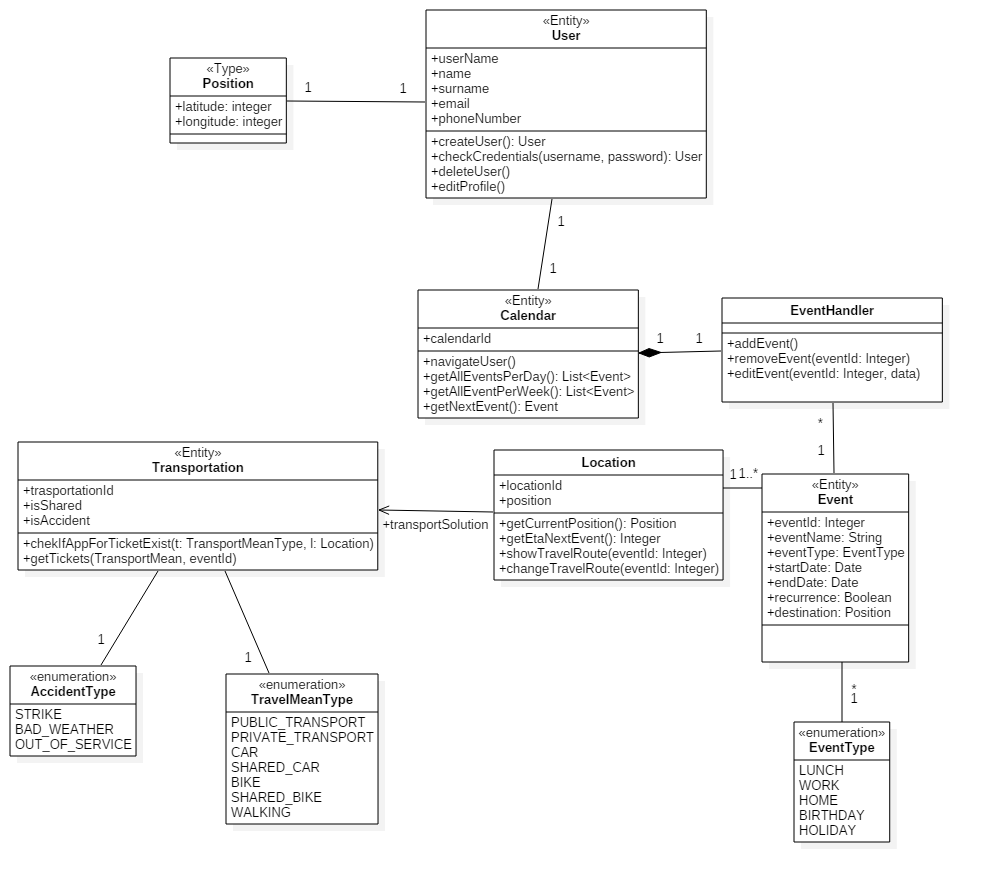
\includegraphics[width=6in]{./diagrams/ClassDiagram.png}
	\caption{Class Diagram}
	\label{fig:seqLogin}
\end{figure}

\subsection*{Specific components}
In detail, these are the main specific components:
\begin{description}
	\item[TravlendarAppGUI:] It provides the user interface to the mobile clients, allowing the usage of the services.
	\item[TravlendarWebGUI:] It provides the user interface to the web-based clients, allowing the usage of the services.
	\item[AuthenticationService:] It is responsible for the identification of the users. It provides the possibility to access the application for existing users or the registration for new users.
	\item[SyncUserInfoService:] It is responsible for the retrieval and synchronization of the user's data across multiple platforms.
	\item[EventService:] It provides the main functionalities of the application. It allows to create, modify and delete events.
	\item[MapService:] It provides the map functionalities and computes the optimal travel route through the best combination of mobility options possible.
	\item[PurchaseService:] It handles the ticket's purchase for the available travel mean. When possible it deep-links the user to the specific application, otherwise it may be redirected to the web-page.
\end{description}

\section{Deployment view}
\label{sec:depl_view}
The following items will cover the major components and technologies that the system uses in order to be deployed to the users.



\section{Runtime view}
\label{sec:runtime_view}
Here we describe the dynamic behavior of the system. In particular, the interaction between the software and the aforementioned logical components interact with each other is shown through sequence diagrams.

\begin{figure}
	\centering
	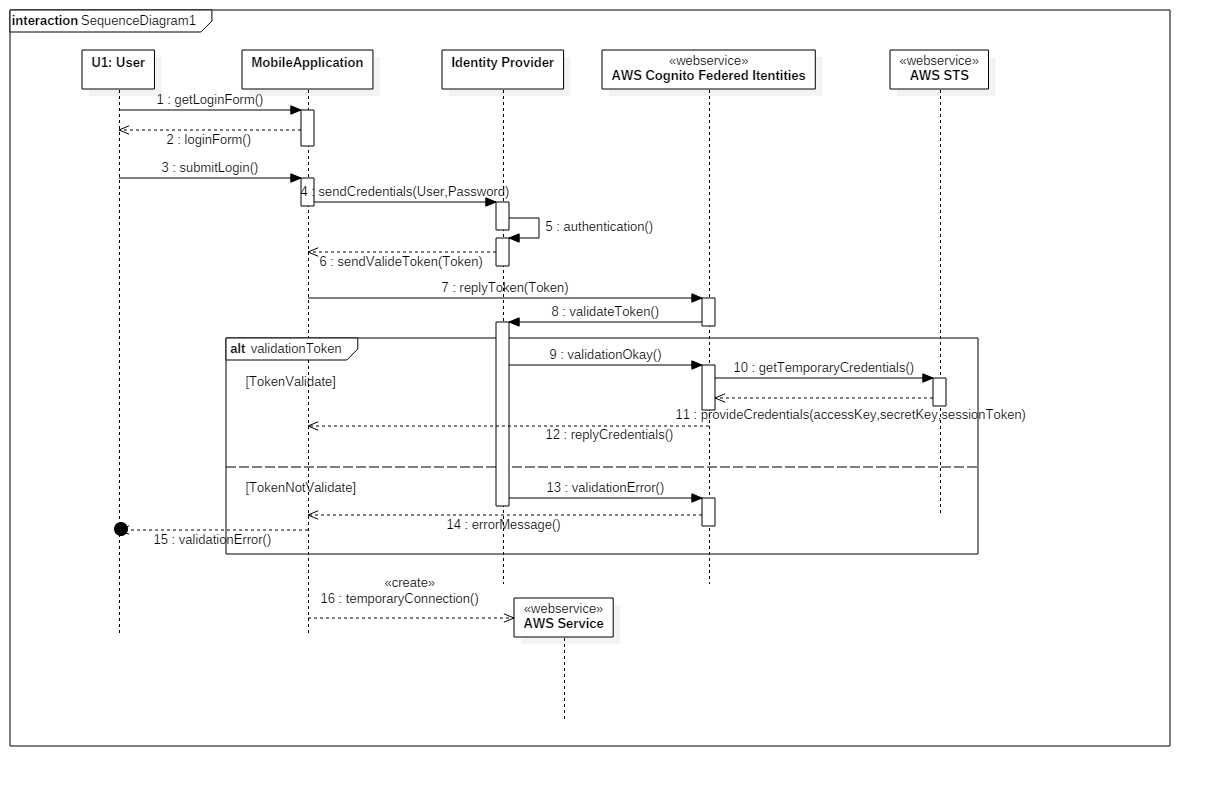
\includegraphics[width=6in]{./diagrams/SequenceDiagramLogin.png}
	\caption{Sequence diagram of the login with the AWS Web Service.}
	\label{fig:seqLogin}
\end{figure}


\begin{figure}
	\centering
	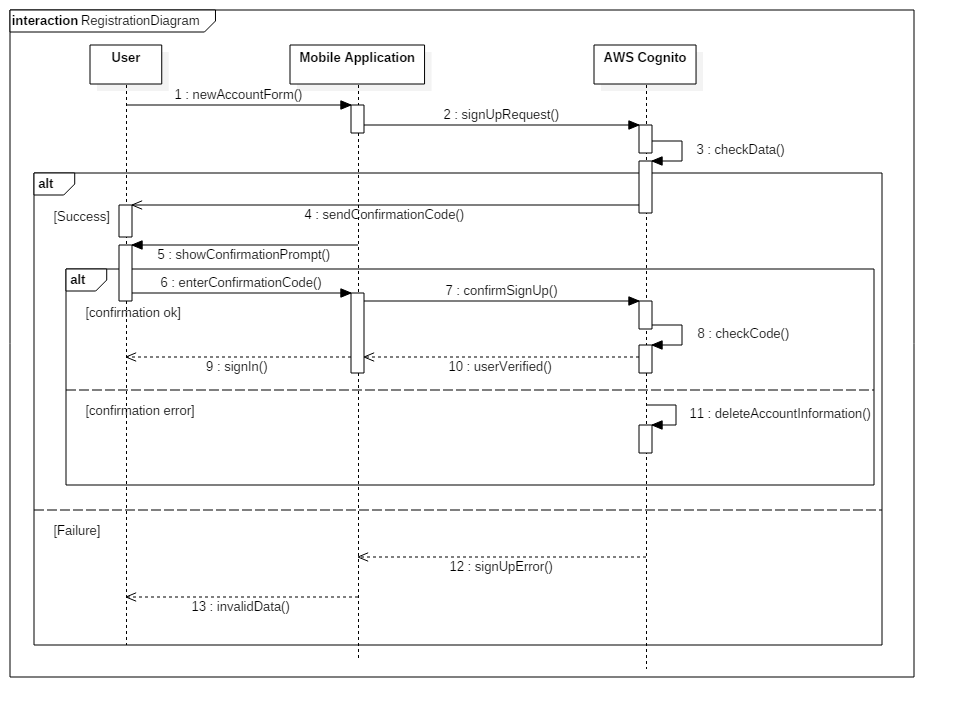
\includegraphics[width=6in]{./diagrams/RegistrationDiagram.png}
	\caption{Sequence diagram of the mobile registration with the AWS Service.}
	\label{fig:seqRegistration}
\end{figure}

\begin{figure}
	\centering
	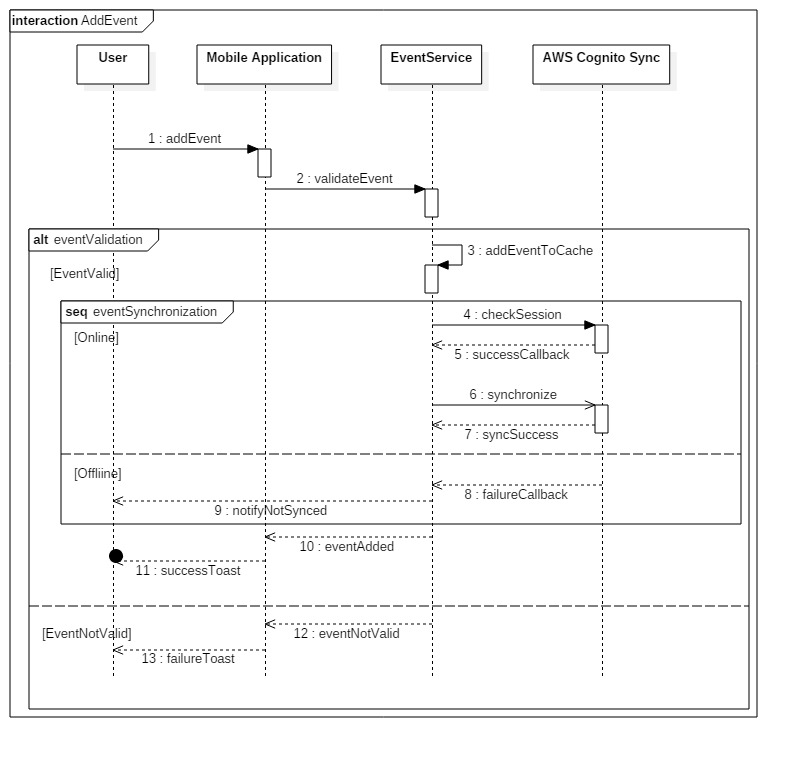
\includegraphics[width=6in]{./diagrams/AddEvent.jpg}
	\caption{Sequence diagram for adding an event.}
	\label{fig:seqAddEvent}
\end{figure}

\begin{figure}
	\centering
	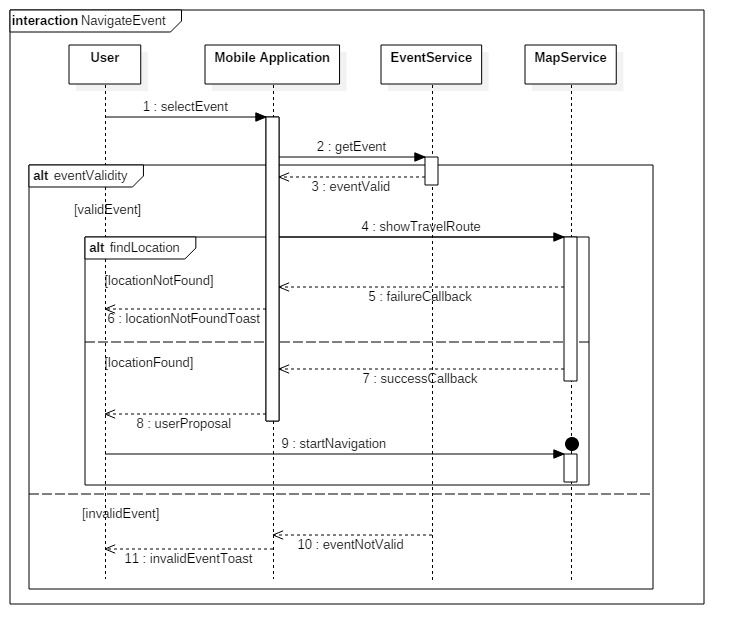
\includegraphics[width=6in]{./diagrams/NavigateEvent.jpg}
	\caption{Sequence diagram for navigating to an event.}
	\label{fig:seqNavigateEvent}
\end{figure}

\section{Component interfaces}
\label{sec:runtime_view}
The following section describes the interfaces by means of which the components communicate with each other. Note that the front-end of the system (both of the mobile application and the web one) must communicate with the application server through RESTful APIs over HTTPS. The RESTful interface is wrapped by AWS SDK in the application server.

\subsubsection*{AuthenticationService}
Methods implemented by the AuthenticationService interface:
\begin{description}
	\item[\texttt{registerUser(info):}] This method creates a new user with AWS Cognito.
	\item[\texttt{loginUser(data):}] This method authenticates an existing user using the AWS Cognito platform.
	\item[\texttt{checkSession(token):}] This method validates the current session with AWS Cognito.
\end{description}

\subsubsection*{UserInformationService}
Methods implemented by the UserInformationService interface:
\begin{description}
	\item[\texttt{synchronizeData(token):}] This method synchronizes the local cache of the AWS Cognito SDK with the AWS Cognito service.
\end{description}

\subsubsection*{EventService}
Methods implemented by the EventService interface:
\begin{description}
	\item[\texttt{addEvent(data):}] This method adds an event to the calendar and synchronizes it with AWS Cognito.
	\item[\texttt{editEvent(eventId, data):}] This method edits a specific event in the calendar and synchronizes it with AWS Cognito.
	\item[\texttt{removeEvent(eventId):}] This method removes a specific event in the calendar and synchronizes it with AWS Cognito.
	\item[\texttt{getEvent(eventId):}] This method returns the given event
	\item[\texttt{getNextEvent():}] This method returns the user's next event.
	\item[\texttt{getAllEventsPerDay():}] This method returns all the events scheduled by the user per day.
	\item[\texttt{getAllEventsPerWeek():}] This method returns all the events scheduled by the user per week.
\end{description}

\subsubsection*{MapService}
Methods implemented by the MapService interface:
\begin{description}
	\item[\texttt{getCurrentPosition():}] This method return current user position.
	\item[\texttt{getETANextEvent():}] This method returns the travel time for the user's next event.
	\item[\texttt{showTravelRoute(eventId):}] This method shows on the map the route for a specific event.
	\item[\texttt{changeTravelRoute(eventId):}] This method attempts to select a different route if the previous one did not satisfy the user.
\end{description}

\subsubsection*{PurchaseService}
Methods implemented by the PurchaseService interface:
\begin{description}
	\item[\texttt{checkIfAppForTicketExist(idTransportMean, location):}] This method checks if there's a third-party application which handles the purchase ticket for a specific transport mean, and if so redirects the user to the application of the dedicated transport mean to buy tickets.
	\item[\texttt{getTickets(idTransportMean, eventId):}] This method retrieves through callbacks the ticket bought by the user on the transport mean application.
\end{description}

\section{Selected architectural styles and patterns}
\label{sec:archs}

Here the main architectural styles and design patterns are identified with the related reason.

\subsection*{Network architecture}
\subsubsection*{Client-server model}
From a network point of view, a well-known structure model is doubtless the client-server one, which is for sure extensively used across networks. Depending on the service provided, such model starts taking place at the following levels:
\begin{itemize}
	\item Mobile application (client) talks to APIs located on the server (when querying for specific data or handling records on the database).
	\item Web application front-end (client) communicates with the server application.
	\item Web server serves pages when user's browser makes a request.
\end{itemize}

\begin{figure}
	\centering
	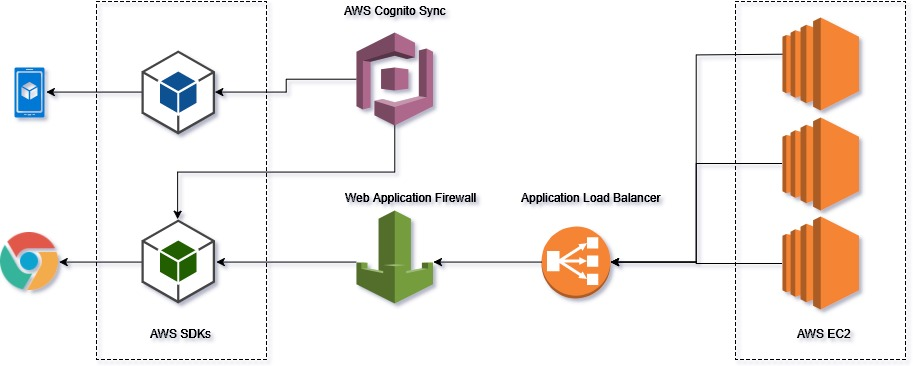
\includegraphics[width=7in]{./diagrams/NetworkDiagram.jpg}
	\caption{Diagram of the network architecture.}
	\label{fig:seqNetworkDiagram}
\end{figure}

\subsection*{Client architecture}
\subsubsection*{MVVM Architectural Pattern}
The Client architecture is based on the pattern Model-View-ViewModel that facilitates the separation of the GUI from the business logic. Being a cross-platform application this will enable a high percentage of shared code across the implementations, speeding the development of the application itself and future features. The primary purpose of MVVM is that the code is broken up into classes with a small number of well-defined responsibilities, serving an easier to understand, maintain and updatable code. Secondly, the MVVM pattern can bring flexibility to the development of the project allowing developers and designer to work simultaneously. It increases as well the application testability, fragmenting and separating the UI logic into different classes from the business logic.
Its a natural pattern for XAML implementations with key enablers like the rich data binding stack and dependency properties. 
This sequence contributes to the connection between the UI/View to the ViewModel.

\subsection*{Design patterns}
\subsubsection*{Inversion of Control and Dependency Injection}

The second major aspect that will characterize the client implementation is the Inversion of Control design paradigm. 
It's a broader concept that aims to give more control to the specific components of the application rather than creating "manually" every object.
Inversion of Control will imply also the Dependency Injection pattern meaning that the approach used to create instances of objects that other objects rely upon without knowing at compile time which classes will provide the functionality itself.
Dependency Injection makes the testing easier, allowing the switch of real service implementation with stubs almost painless.
These aspects are compliant with the GRASP guidelines, specifically in the High Cohesion evaluative pattern.
It attempts to keep objects properly directed on their goal developing the whole system into a low coupling system with several classes and subsystems.

\subsubsection*{Separation of Concerns}
Strictly related to the already mentioned patterns, we include also a principle of fundamental importance in order to achieve separation of our application into several distinct features that overlap in functionality with minimum "interference" possible. MVVM pattern perfectly allows us to achieve such principle, known as separation of concerns. By means of information hiding (which is realized with encapsulation), every module will have its own interface to communicate with each other and hide the internal business logic. More specifically, in the context of MVVM, Views do not know (almost) nothing about each other, especially what is going on in the ViewModel, which contains, as said, the workflow of the application and connects the UI with the business logic itself through data binding. Just to mention some benefits we can obtain are surely maintainability and reusability.

\section{Other design decisions}
\label{sec:des_dec}
The user's credentials are not stored in the device, rather the AWS SDK provides a way to save the tokens used to access the AWS Services. Those tokens will be hashed and stored in an AES encrypted SQLite database. The key to access it is generated upon the installation of the application, providing a unique random key stored in the respective Keystore/Keychain platform implementations. Travlendar+ will rely on Google Maps for everything that concerns the route calculation and map implementations on the clients. Being a leader in the field, it provides a wide support to the APIs integrations as well as for the SDK to be implemented on the clients.
It helps to delegate much of the effort to a well-established component in which the users can feel comfortable to use.